\subsection{A controlled quadrupole-coupling path}

To isolate a dynamical origin, we varied the $^{135}$Ba quadrupole coupling as
$\Gamma_0=0.6s$ MeV, with $s=0,0.25,0.50,0.75,1$, while keeping the exchange
and monopole strengths, core, occupation and charge operator fixed.
These are interventions in the model, not alternative fits to the nucleus.
Forward and backward maximum-overlap tracking both select the lowest
$11/2$ state throughout the sampled path. Adjacent squared overlaps exceed
0.907, and the smallest sampled gap to the next state of the same spin is
0.481 MeV. Thus no lowest-state switch is observed at this resolution.

Figure~\ref{fig:path} shows a strong redistribution with little change in total
strength. Complete $q_2$ remains between 0.67662 and
$0.69413\,e^2{\rm b}^2$, a range of less than $2.6\%$, and
$\langle n_d\rangle$ stays between 2.324 and 2.354. The static fraction,
however, rises from $0.0091\%$ to $33.69\%$. The core-$R=2$ probability
increases from 0.0151 to 0.4837, while the core-$R=0$ probability falls
from 0.9522 to 0.4886. In this controlled comparison, quadrupole coupling
principally changes angular recoupling and static polarization rather than
the amount of quadratic charge strength.

\begin{figure*}[t]
\centering
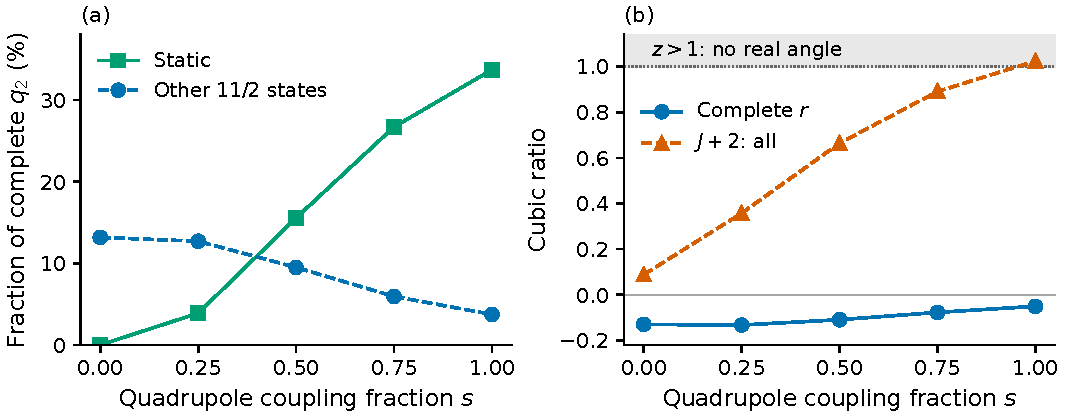
\includegraphics[width=\textwidth]{figures/quadrupole_path-v2.pdf}
\caption{Fixed-exchange/monopole control for $^{135}$Ba:
$\Gamma_0=0.6s$ MeV, $\Lambda_0=1$ MeV, $A_0=-0.9$ MeV.
The core and electric-quadrupole operator are unchanged.
(a) Static and other-same-spin fractions of complete $q_2$.
(b) Complete signed ratio and the all-$15/2$ selected ratio.
Points are the five calculated settings; lines guide the eye.
The shaded region has no real selected angle.}\label{fig:path}
\end{figure*}

The selected ratio rises through a specific change of its numerator and
denominator. Over the path, $S_\infty$ falls from 2.32070 to
$1.62594\,e^2{\rm b}^2$, whereas the signed chain $C_\infty$ grows from
0.37162 to $2.53787\,e^3{\rm b}^3$. In the intermediate energy eigenbasis,
its middle-diagonal contribution changes from
$-0.73467$ to $+1.16709\,e^3{\rm b}^3$: cancellation with off-diagonal
paths is replaced by reinforcement. Consequently $z_\infty$ rises from
0.08795 to 1.02414. At the final point, the additional spin sectors in the
complete cubic moment still largely cancel. Since the all-$15/2$ projector
is unchanged along this path, the result is a change of the initial
state's charge response, not a consequence of reordering a five-state list.

\subsection{Charge-operator and static-moment constraints}\label{sec:emlimits}

The distinction between channel saturation and full coverage survives
35 operator/calibration settings, evaluated on the fixed Ba states:
the primary setting, two fermion charges, two alternative $\chi'$ values
and both quoted-margin core-strength endpoints for each isotope.
Across these settings, the full $15/2$ channel carries 14.12--29.24\%
of $q_2$, and its first five states exhaust 99.588--99.939\% of that channel.
These are deterministic sensitivity tests, not a parameter posterior.

The actual cubic coordinates are more sensitive. In $^{135}$Ba,
$\chi'=0$ or $\chi'=\chi=-0.24$ removes the selected-domain failure and
changes the complete cubic sign. The complete/selected folded angles
become $24.418^\circ/6.241^\circ$ and
$20.166^\circ/10.659^\circ$, respectively. Changing an E2 operator on
one wavefunction is not a change of Hamiltonian shape.

Static moments further constrain nuclear interpretation.
The primary $^{137}$Ba value, $Q_s=+0.77296\,e\,{\rm b}$, agrees with
its source-named calibration target $+0.78(9)\,e\,{\rm b}$ and is not
an independent test. The $^{135}$Ba prediction,
$+1.17693\,e\,{\rm b}$, exceeds the evaluated $+0.96(8)\,e\,{\rm b}$;
Ref.~\cite{Nomura2017} separately quotes $+0.98(8)$ experimentally
and $+1.13\,e\,{\rm b}$ theoretically. The source variants are not averaged.
The primary $^{136}$Ba core moment also disagrees with several evaluated
calibration branches. These discrepancies limit the quantitative static
redistribution that can be assigned to the actual nucleus.

We retained all five finite central-value operator calibrations obtained
from the distinct $^{136}$Ba moment targets, the common core strength
and $Q_s(^{137}{\rm Ba})=0.78\,e\,{\rm b}$, without using $^{135}$Ba to
select a branch. Two branches improve its predicted moment to 0.923 and
$0.915\,e\,{\rm b}$ but give complete ratios $r=-1.093$ and $-1.096$.
Thus even complete moments need not admit a real rigid-equivalent angle.
Appendix~\ref{app:calibrated} retains every branch, the shared-source
and unknown-covariance limitations, and a marginal truncation case.
Matching $Q_s$ through the coupling instead changes the spectrum
(Appendix~\ref{app:momentmatch}); neither calibration is an independent
validation of the electromagnetic network.
